\documentclass[9pt,twocolumn,twoside]{pnas-new}
% Use the lineno option to display guide line numbers if required.
% Note that the use of elements such as single-column equations
% may affect the guide line number alignment. 

\templatetype{pnasresearcharticle} % Choose template 
% {pnasresearcharticle} = Template for a two-column research article
% {pnasmathematics} = Template for a one-column mathematics article
% {pnasinvited} = Template for a PNAS invited submission
\usepackage{siunitx}
\setcitestyle{authoryear,open={(},close={)}}

\setboolean{displaywatermark}{false} % Set to false to remove the watermark

\title{Bestimmung der Spurabstände von optischen Datenträger}

% Use letters for affiliations, numbers to show equal authorship (if applicable) and to indicate the corresponding author
\author[a]{Armin Beck}
\author[a]{André Berberich} 
\author[a]{Fabian Konrad}

\affil[a]{Student der DHBW Mosbach}


% Keywords are not mandatory, but authors are strongly encouraged to provide them. If provided, please include two to five keywords, separated by the pipe symbol, e.g:
\keywords{Laser $|$ CD $|$ DVD $|$ Storage} 

\begin{abstract}
This paper presents a revolutionary and repeatable method to prove the track pitch of an optical, laser based, data medium.
Using a hand held light emitting pistol, the track pitch of an standard medium was measured to be between 0,73 \textmu m and 1,6  \textmu m.
Results show outstanding agreement with the provided, theoretical values of the manufacturers.
The method presented has significant implications for future storage of big data in the cloud 
and may one day will be the contributing factor for the digitization of the industry.
\end{abstract}

\dates{This manuscript was compiled on \today}

\begin{document}

% Optional adjustment to line up main text (after abstract) of first page with line numbers, when using both lineno and twocolumn options.
% You should only change this length when you've finalised the article contents.
\verticaladjustment{-2pt}

\maketitle
\thispagestyle{firststyle}
\ifthenelse{\boolean{shortarticle}}{\ifthenelse{\boolean{singlecolumn}}{\abscontentformatted}{\abscontent}}{}

\dropcap{D}ie Forschung ist sich einig, dass es wichtig ist, bestehende Technologien zu reflektieren und daraus entsprechende Schlüsse für die Zukunft zu ziehen. Weiterentwicklungen im Speicherbereich dienen als Grundlage für den Weg der Digitalisierung und der globalen Vernetzung. 
Die Anforderungen an Speicher, der jederzeit erreichbar, redundant ausgelegt und hochperformant sein muss, steigt mit jedem Tag.
Auch Privatanwender sind von diesem \glqq recht abrupte[n] Paradigmenwechsel\grqq \space betroffen \cite[Heft 10/2012 S.102]{CT1990}.
Die in diesem Artikel vorgestellte Methode ermöglicht es Spurabstände auf optischen Datenträgern mit einfachsten Mitteln zu bestimmen und zu validieren, ohne hierbei einen Computer oder ein Laufwerk zu verwenden. Dies ermöglicht es, siginfikante Unterschiede diverser optischer Medien im Bezug auf die Datenkapazität, zu erklären. Durch diese Vorgehensweise ermittelten Werte für handelsübliche CDs und DVDs, sollen als Referenz und Denkanstoß für die Entwicklung von innovativen Speicherlösungen von morgen dienen.

\section*{Technische Grundlagen der Methode}
Bei diesem Verfahren werden die Effekte eines von elektromagnetischen Wellen bestrahlten Doppelspalts genutzt.
 Wird eine Lochplatte, beziehungsweise eine Spaltplatte, von einem Laserstrahl getroffen, so verteilt sich das Licht nahezu gleichmäßig hinter der Platte.
 Durch eine Mattscheibe hinter dem Doppelspalt, sind mehrere von der Mitte aus symmetrisch angeordnete Punkte in zunehmendem Abstand zur Mitte sichtbar.
Dies scheint keiner gleichmäßigen Verteilung zu entsprechen, allerdings streuen zwei Spalten den Lichtstrahl.
Wird ein Punkt in einem Abstand von beiden Löchern betrachtet, der sich um jeweils \begin{math}n\cdot\lambda\end{math} unterscheidet, ist an diesem die Bestrahlungsstärke höher, da die aus beiden Spalten austretenden Wellen an dieser Stelle nicht zueinander phasenverschoben sind. Ein sogenanntes Interferenzmaximum entsteht aus der Addition der Amplituden beider austretender Wellen. An anderen Stellen tritt eine Phasenverschiebung auf, da die Lichtstrahlen an unterschiedlichen Punkten der Periode zusammentreffen. Somit entsteht eine von der Position abhängige stehende Welle, die durch die Mattscheibe visualisiert wird.

\subsection*{Aufbau und Leseverfahren einer CD und einer DVD}
CDs und DVDs bestehen grundsätzlich aus drei Schichten. Die unterste Schicht ist eine Kunststoffscheibe, auf der die Binärdaten in Form von Vertiefungen eingeprägt bzw. mit einem Laser eingebrannt wurden. Die zweite Schicht ist eine Metallfolie, die zur Reflektion dient. Die dritte Schicht ist eine bedruckte Schutzfolie, welche die darunterliegende Metallfolie und Kunststoffscheibe schützt. Zum Lesen wird die Unterseite von einem Laserstrahl beleuchtet. Dabei wird der Strahl von der Metallfolie reflektiert und von einem Sensor erfasst. Trifft der Strahl auf eine Vertiefung, wird er reflektiert und trifft den Sensor mit geringerer Intensität. Durch Messung der Intensität können die Daten gelesen und weiterverarbeitet werden.

\section*{Exemplarische Durchführung}

\begin{figure}[!htbp]
\centering
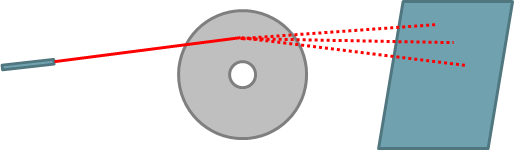
\includegraphics[width=0.3\textwidth,keepaspectratio]
{Pictures/Versuchsaufbau.png}
\parbox{0.9\textwidth}

{\caption{\label{fig:Versuchsaufbau}
exemplarischer Aufbau}
\sffamily \small{Ein Laserstrahl wird auf den Datenträger gerichtet. Die durch den Datenträger abgelenkt und reflektierten Strahlen werden auf einer Mattscheibe visualisiert.}
}
\end{figure}

Aufgrund der Funktionsweise des Leseverfahrens, ist es naheliegend, ein ähnliches Verfahren zur Ermittlung des Spurabstandes von optischen Datenträgern zu nutzen. Dabei können die Vertiefungen in der Kunststoffschicht als Doppelspalt genutzt werden. Um davon auf den Spurabstand schließen zu können, ist es erforderlich, dass mehrere Löcher auf mindestens zwei verschiedenen Spuren simultan bestrahlt werden. Wenn mehrere Spuren bestrahlt werden, treten keine für die Messung negativen Effekte auf \cite{Kit2016Dreifachspalt}. Wegen des daraus resultierenden Größenverhältnisses zwischen Spurabstand und Strahlgröße ist es notwendig, einen Laserstrahl zu verwenden, der breit genug ist. Ein handelsüblicher Laserpointer erfüllt diese Voraussetzungen. Zur Erfassung der abgelenkten und reflektierten Strahlen wird eine Mattscheibe genutzt, auf welcher die Abstände der Strahlen zueinander gemessen werden können. Daraus ergibt sich der in Fig.\ref{fig:Versuchsaufbau} vereinfacht dargestellte Aufbau.



\begin{figure}[!htbp]
\centering
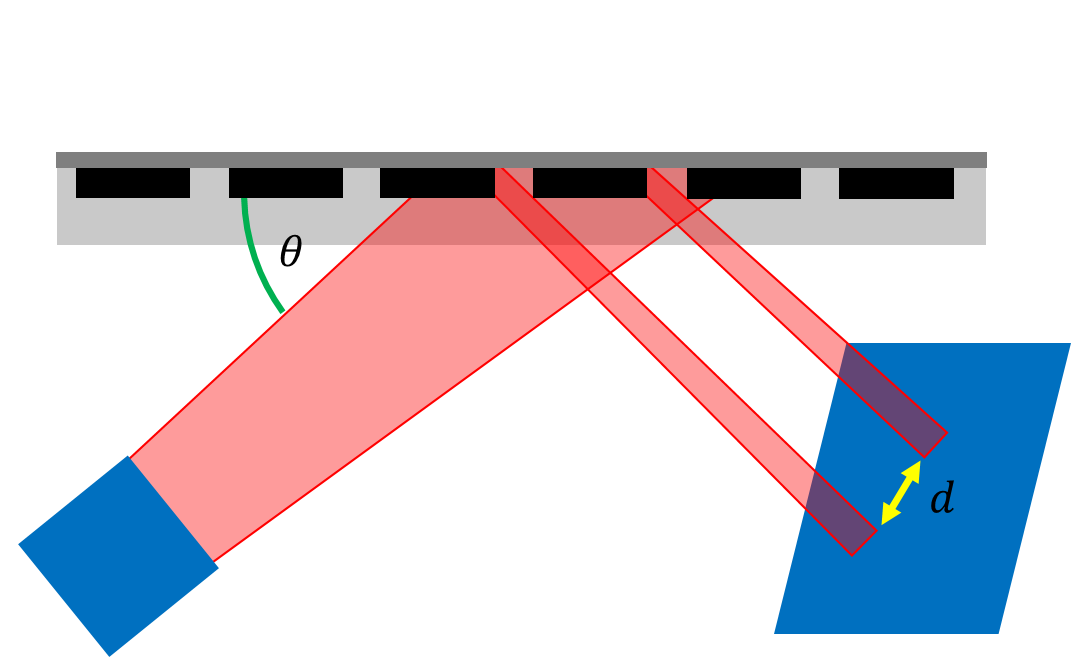
\includegraphics[width=0.3\textwidth,keepaspectratio]
{Pictures/Spalt.png}
\parbox{0.9\textwidth}

{\caption{\label{fig:Spalt}
Doppelspalteffekt am vom Laser angestrahlten optischen Datenträger}
\sffamily \small{
Der auf den Datenträger flach auftreffende Laserstrahl wird abgelenkt und von Vertiefungen unterschiedlicher Spuren auf die Mattscheibe reflektiert. Der Abstand der Strahlen ist auf der Mattscheibe messbar.}
}
\end{figure}



\section*{Exemplarische Ergebnisse}
Da die Vertiefungsabstände von CD und DVD sehr gering sind, kann man die vom Laserpointer beleuchtete Stelle als Doppelspalt betrachten (Siehe Fig.\ref{fig:Spalt}). Es treten die oben genannten Interferenzeffekte auf, anhand deren gemäß \cite{Kit2016Doppelspalt} das Verhältnis aus der gegebenen Wellenlänge des Lasers \begin{math}\lambda[\mbox{nm}]\end{math} und dem Vertiefungsabstand berechnet werden kann. Hierbei wird zuerst aus dem gemessenen Abstand der Interferenzmaxima \begin{math}d[\mbox{cm}]\end{math} und dem Abstand zwischen Mattscheibe und Datenträger \begin{math}l[\mbox{cm}]\end{math} der Austrittswinkel \begin{math}\theta\end{math} berechnet. Die Berechnung hierzu erfolgt über den Arcustangens:

\begin{equation}
\label{eq:Theta_Berechnung}
\theta=\arctan\frac{d}{l}.
\end{equation}

Aus diesem Winkel lässt sich nun entsprechend Fig.\ref{fig:Doppelspalt_Modell} mit Hilfe des Gangunterschieds \begin{math}\Delta s[\mbox{nm}]\end{math} der Spurabstand \begin{math}g[\mbox{\textmu m}]\end{math} berechnen. Der Gangunterschied kann in diesem Fall gleich der Wellenlänge \begin{math}\lambda[\mbox{nm}]\end{math} gesetzt werden, da ein Interferenzmaximum nur auftritt, wenn die beiden Wellen im gleichen Phasenabschnitt auftreten.
Daraus wird nun die Berechnungsformel für den Spurabstand abhängig von Wellenlänge und Winkel abgeleitet:

\begin{equation}
\label{eq:Spurabstand_Sinus}
 g= \frac{\Delta s}{\sin\theta}= \frac{\lambda}{\sin\theta}.
\end{equation}

\begin{figure}[!htbp]
\centering
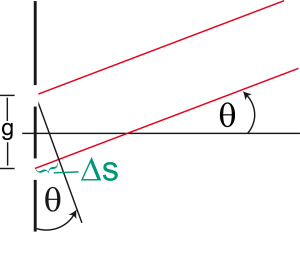
\includegraphics[width=0.3\textwidth,keepaspectratio]
{Pictures/Doppelspalt_Modell.png}
\parbox{0.9\textwidth}

{\caption{\label{fig:Doppelspalt_Modell}
Ablekungsmodell am Doppelspalt}

\sffamily \small{Der Winkel \begin{math}\theta\end{math} stellt die Ablenkung des Lichtstrahls gegenüber dem Doppelspalt dar.  \begin{math}\Delta s =\end{math} ist der Gangunterschied. \cite{kit2016}}
}
\end{figure}

\begin{table}[!tbhp]
\centering
\caption{Messergebnisse in Abhängigkeit verschiedener Abstände}
\label{table:results}
\begin{tabular}{lrrrrrr}
\begin{math} l \mbox{ in cm} \end{math} & 10 & 12 & 14 & 16 & 18 & 20 \\
\midrule
\begin{math}d_{\mbox{cd}} \mbox{ in cm} \end{math} & 3,8 & 4,6 & 5,3 & 6,1 & 6,9 & 7,6 \\
\begin{math}d_{\mbox{dvd}} \mbox{ in cm} \end{math} & 17,3 & 20,8 & 24,1 & 27,7 & 31,1 & 34,6 \\
\begin{math}\theta_{\mbox{cd}} \mbox{ in Grad} \end{math}& 20,8 & 21,0 & 20,7 & 20,9 & 21,0 & 20,8 \\
\begin{math}\theta_{\mbox{dvd}} \mbox{ in Grad} \end{math} & 60,0 & 60,0 & 59,9 & 60,0 & 59,9 & 60,0  \\
\bottomrule
\end{tabular}

\sffamily \small \addtabletext{Gemessene Abstände für die CD und DVD sowie die daraus berechneten Ablenkungswinkeln}
\end{table}

Für den Spurabstand einer CD ergibt sich dann mit \eqref{eq:Spurabstand_Sinus} und der Wellenlänge des verwendeten Lasers(632\si{\nano\metre}) sowie einem exemplarischen Wert aus Tabelle \ref{table:results}:
\begin{align*}
 g_{cd} &= \frac{632\cdot10^{-9}\mbox{m}}{\sin{20,8\mbox{\textdegree}}}\\
 &\approx 1,78 \cdot 10^{-9}\mbox{m}
\end{align*}
Analog dazu der Spurabstand der DVD mit \eqref{eq:Spurabstand_Sinus}:
\begin{align*}
 g_{dvd} &= \frac{632\cdot10^{-9}\mbox{m}}{\sin{60,0\mbox{\textdegree}}}\\
 &\approx 0,73 \cdot 10^{-9}\mbox{m}
\end{align*}


\section*{Interpretation der ermittelten Werte}
Durch die gewonnen Messergebnisse konnten die Hersteller Angaben von 0,73 \si{\micro\metre} (DVD) \cite{ECMA1300} und  1,6 \si{\micro\metre} (CD) \cite{ECMA359} bestätigt werden.
\begin{equation} \label{eq:cdspur} S_{\mbox{cd }} =  1,78\mbox{ \textmu m} \end{equation} 
\begin{equation} \label{eq:dvdspur} S_{\mbox{dvd}} =  0,73\mbox{ \textmu m}  \end{equation} 
\subsection{Vergleich Datenkapazität CD und DVD}
Der geringere Spurabstand der DVD ist einer der Gründe, warum diese eine höhere Datenkapazität als die CD hat, obwohl beide die gleiche Bauform haben.

\begin{figure}[!htbp]
\centering
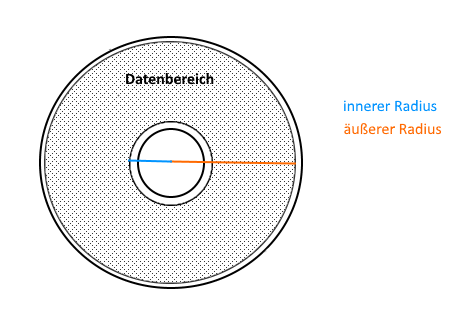
\includegraphics[width=0.5\textwidth,keepaspectratio]
{Pictures/Rohling.png}
\parbox{0.9\textwidth}

{\caption{\label{fig:Rohling}
Schematische Darstellung eines optischen Datenträgers}

\sffamily \small{Ein typischer optischer Datenträger mit gekennzeichneten Radien zur Darstellung des Datenbereichs}
}
\end{figure}

Aus Fig.\ref{fig:Rohling}, das den schematischen Aufbau eines optischen Datenträgers zeigt, können zwei Radien entnommen werden, über die die Fläche des Datenbereichs berechnet werden kann.
Für die folgenden Berechnungen gilt: \begin{align*} r_{\mbox{i}}  = \mbox{innerer Radius und } r_{\mbox{a}} = \mbox{äußerer Radius} \end{align*} 


Mit der Formel für die Fläche eines Kreisringes \cite[Seite 147]{Bartsch2014} kann die Fläche für Daten berrechnet werden: \begin{equation} \label{eq:kreisring} A = \pi((r_a)^2-(r_i)^2).  \end{equation}

Die Gesamtlänge einer Spur kann folgendermaßen berechnet werden \begin{equation} \label{eq:gesamtlänge} L = \frac{\mbox{Fläche für Daten}}{\mbox{Spurabstand}}. \end{equation}
Die Anzahl der Bits im Datenbereich kann anschließend näherungsweise berechnet werden (unter Berücksichtigung des Spurabstandes) \begin{equation} \label{eq:bitanzahl} N_{bits} = \frac{L}{0,5*\mbox{Spurabstand}}. \end{equation}

\subsection{Berechnung CD}
Von einer CD konnten folgende Werte abgelesen werden:
\begin{align*}
 r_{\mbox{i}_{\mbox{cd}}} &= 2,3 \mbox{ cm und } r_{\mbox{a}_{\mbox{cd}}} = 5,8 \mbox{ cm}
 \end{align*} 
\indent Die Datenfläche errechnet sich aus \eqref{eq:kreisring}:
\begin{align*}
 A_{cd} &= \pi\cdot((r_{\mbox{a}_{\mbox{cd}}})^2-(r_{\mbox{i}_{\mbox{cd}}})^2)\\	
&= \pi\cdot((5,8\mbox{cm})^2-(2,3\mbox{ cm})^2) \\
 &=  \pi\cdot((0,058\mbox{ m})^2-(0,023\mbox{ m})^2) \\
 &\approx  8,91\cdot10^{-3}\mbox{ m}^2.
\end{align*}

Die Länge der Spur ergibt sich aus \eqref{eq:kreisring} mit \eqref{eq:cdspur}:
\begin{align*}
 L_{cd} &= \frac{\mbox{Fläche für Daten}}{\mbox{Spurabstand}}\\
 &= \frac{A_{\mbox{cd}}}{S_{\mbox{cd}}}\\
 &= \frac{8,91\cdot10^{-3}\mbox{ m}^2}{1,78\cdot10^{-6}\mbox{ m} }\\
 &= 5005\mbox{ m}.
\end{align*}

Die Anzahl der Bits beträgt dann über \eqref{eq:bitanzahl}:
\begin{align*}
N_{\mbox{cd-bits}} &=  \frac{L_{\mbox{cd}}}{0,5\cdot s_{\mbox{cd}}}\\
&= \frac{5005\mbox{ m}}{0,5 \cdot 1,78 \cdot 10^{-6}\mbox{ m}}\\
&\approx 5,6 \cdot 10^9.
\end{align*}

Umgerechnet in MiB:
\begin{align*}
C_{\mbox{cd}} &= \frac{N_{\mbox{cd-bits}}}{8\cdot1024\cdot1024}\\
&= \frac{ 5,6\cdot10^9}{8\cdot1024\cdot1024}\\
&\approx 668\mbox{ MiB}.
\end{align*}

Die Größenordnung entspricht der einer handelsüblichen CD.

\subsection{Berechnung DVD}
Von einer DVD konnten die folgenden Werte abgelesen werden: 
\begin{align*}
 r_{\mbox{i}_{\mbox{dvd}}} = 2,3 \mbox{ cm und } r_{\mbox{a}_{\mbox{dvd}}} = 5,9 \mbox{ cm} 
\end{align*}

\indent Die Datenfläche errechnet sich aus \eqref{eq:kreisring}:
\begin{align*}
 A_{\mbox{dvd}} &= \pi\cdot((r_{\mbox{a}_{\mbox{dvd}}})^2-(r_{\mbox{i}_{\mbox{dvd}}})^2)  \\	
&= \pi\cdot((5,9\mbox{cm})^2-(2,3\mbox{ cm})^2) \\
 &=  \pi\cdot((0,059\mbox{ m})^2-(0,023\mbox{ m})^2) \\
 &\approx 9,27\cdot10^{-3}\mbox{ m}^2.
\end{align*}

Für die Länge der Spur aus \eqref{eq:kreisring} ergibt sich mit \eqref{eq:dvdspur}:
\begin{align*}
 L_{\mbox{dvd}} &= \frac{\mbox{Fläche für Daten}}{\mbox{Spurabstand}}\\
 &= \frac{A_{\mbox{dvd}}}{S_{\mbox{dvd}}}\\
 &= \frac{9,27\cdot10^{-3}\mbox{ m}^2}{0,73\cdot10^{-6}\mbox{ m} }\\
 &\approx 12700\mbox{ m}.
\end{align*}

Die Anzahl der Bits beträgt dann über \eqref{eq:bitanzahl}:
\begin{align*}
N_{\mbox{dvd-bits}} &=  \frac{L_{\mbox{dvd}}}{0,5\cdot S_{\mbox{dvd}}}\\
&= \frac{12700\mbox{ m}}{0,5\cdot 0,73\cdot10^{-6}\mbox{ m}}\\
&\approx 3,48\cdot 10^{10}.
\end{align*}

Umgerechnet in GiB:
\begin{align*}
C_{\mbox{dvd}} &= \frac{N_{\mbox{dvd-bits}}}{8\cdot1024\cdot1024\cdot1024}\\
&= \frac{3,48\cdot10^{10}}{8\cdot1024\cdot1024\cdot1024}\\
&\approx 4,05\mbox{GiB}.
\end{align*}
\\\\
Auch diese Größenordnung entspricht der einer handelsüblichen DVD.\\
Mit dieser Methode ist es nun auch möglich, weitere optische Datenträger zu überprüfen.
Aufgrund der erhebbaren Daten sind Neuerungen in der Speichertechnik von optischen Medien denkbar, die in der Zukunft eine zentrale Rolle für Speicherlösungen spielen können. Heute sind bereits optische Datenträger mit bis zu 1 TB in Entwicklung \cite{SonyPressStatement}.
\\
% \pnasbreak splits and balances the columns before the references.
% Uncomment \pnasbreak to view the references in the PNAS-style
% If you see unexpected formatting errors, try commenting out \pnasbreak
% as it can run into problems with floats and footnotes on the final page.
%\pnasbreak
% Bibliography
\bibliography{ReferenceDatabase}


\end{document}
